% !TEX root = ./4-Integrales_Multiples_Slides.tex

%!! To Do: 
%!  Reconstruir imágenes:
%!  - región elemental 3D
%!  - cambio de variables a coordenadas cilíndricas
%!  - cambio de variables a coordenadas esféricas

%! Datos del curso
\newcommand{\SIGLACURSO}{MAT013}
\newcommand{\NOMBRECURSO}{Matemática 3}
\newcommand{\PROFESOR}{Eduardo Hirsh}
\newcommand{\FECHA}{Primer Semestre 2026}
\newcommand{\FECHACORTO}{1er. Semestre 2026}

%! Datos presentación
\newcommand{\NOMBREDOCUMENTO}{Integrales Múltiples}
\author{\PROFESOR}
\title[\SIGLACURSO]{\SIGLACURSO\ - \NOMBRECURSO\\ \NOMBREDOCUMENTO}
\date[\FECHACORTO]{\FECHA}
\institute[]{}

%! Configuración de las enumeración
% facilita la personalización de listas funciona mejor en article
% \usepackage[shortlabels]{enumitem}
\setbeamertemplate{enumerate items}{\arabic{enumi}.}
\setbeamertemplate{enumerate subitem}{\alph{enumii})}
\setbeamertemplate{enumerate subsubitem}{\roman{enumiii}.}

\begin{document}

\only<article>{
%! Encabezado
\thispagestyle{empty}
\vspace*{-4cm}
\begin{center}
  
\includegraphics[scale=.75]{logo-dmat-vertical.pdf}
\end{center}
% \vspace{1mm}
% \noindent\rule[0mm]{175mm}{0.1mm}

%! Titulo
\begin{center}
  \textbf{\Large\SIGLACURSO\ - \NOMBRECURSO}\\[1mm]
  \textbf{\Large\NOMBREDOCUMENTO}\\
  {\large\PROFESOR}\\
  \FECHACORTO
\end{center}
\vspace{5mm}
}

\only<presentation>{
\begin{frame}
  \begin{center}
  
\includegraphics[scale=.6]{Logo_USM_MAT.pdf}
  \end{center}
  \titlepage
  % \begin{center}\includegraphics[scale=.20]{Logo_Depto.pdf}\end{center}
  \vspace{2cm}
\end{frame}
}

%! tabla de contenidos completa
\begin{frame}
\tableofcontents
\end{frame}

%! sección
\section{Integrales Dobles}
\begin{frame}
\sectionpage
\end{frame}

\begin{frame}
\tableofcontents[currentsection]
\end{frame}

%! subsección
\subsection{Sumas de Riemann Sobre Rectángulos}
\begin{frame}
\subsectionpage
\end{frame}

% \begin{frame}
% \tableofcontents[currentsubsection]
% \end{frame}

\begin{frame}
  Una región rectangular cerrada es una región de la forma.
  $$R=\set{(x,y)\in\Real^2:a\leq x\leq b\wedge c\leq x\leq d}$$
  \onslide<2->{También lo anotaremos como
  $$R=[a,b]\times[c,d]=\set{(x,y):x\in[a,b]\wedge y\in[c,d]}$$
  }
\end{frame}

\begin{frame}
  $$R=[a,b]\times[c,d]$$
  \onslide<2->{$$x_0=a<x_1<x_2<\ldots<x_m=b$$ $$y_0=c<y_1<y_2<\ldots<y_n=d$$}
  \onslide<3->{$$R_{ij}=[x_{i-1},x_i]\times[y_{j-1},y_j]$$}
  \onslide<4->{$$(x_i^*,y_j^*)\in R_{ij}$$}
  \onslide<5->{$$\Delta x_i=x_i-x_{i-1}$$ $$\Delta y_j=y_j-y_{j-1}$$ $$\Delta A_{ij}=\Delta x_i\Delta y_j$$}
\end{frame}

\begin{frame}
\begin{figure}
\begin{center}
  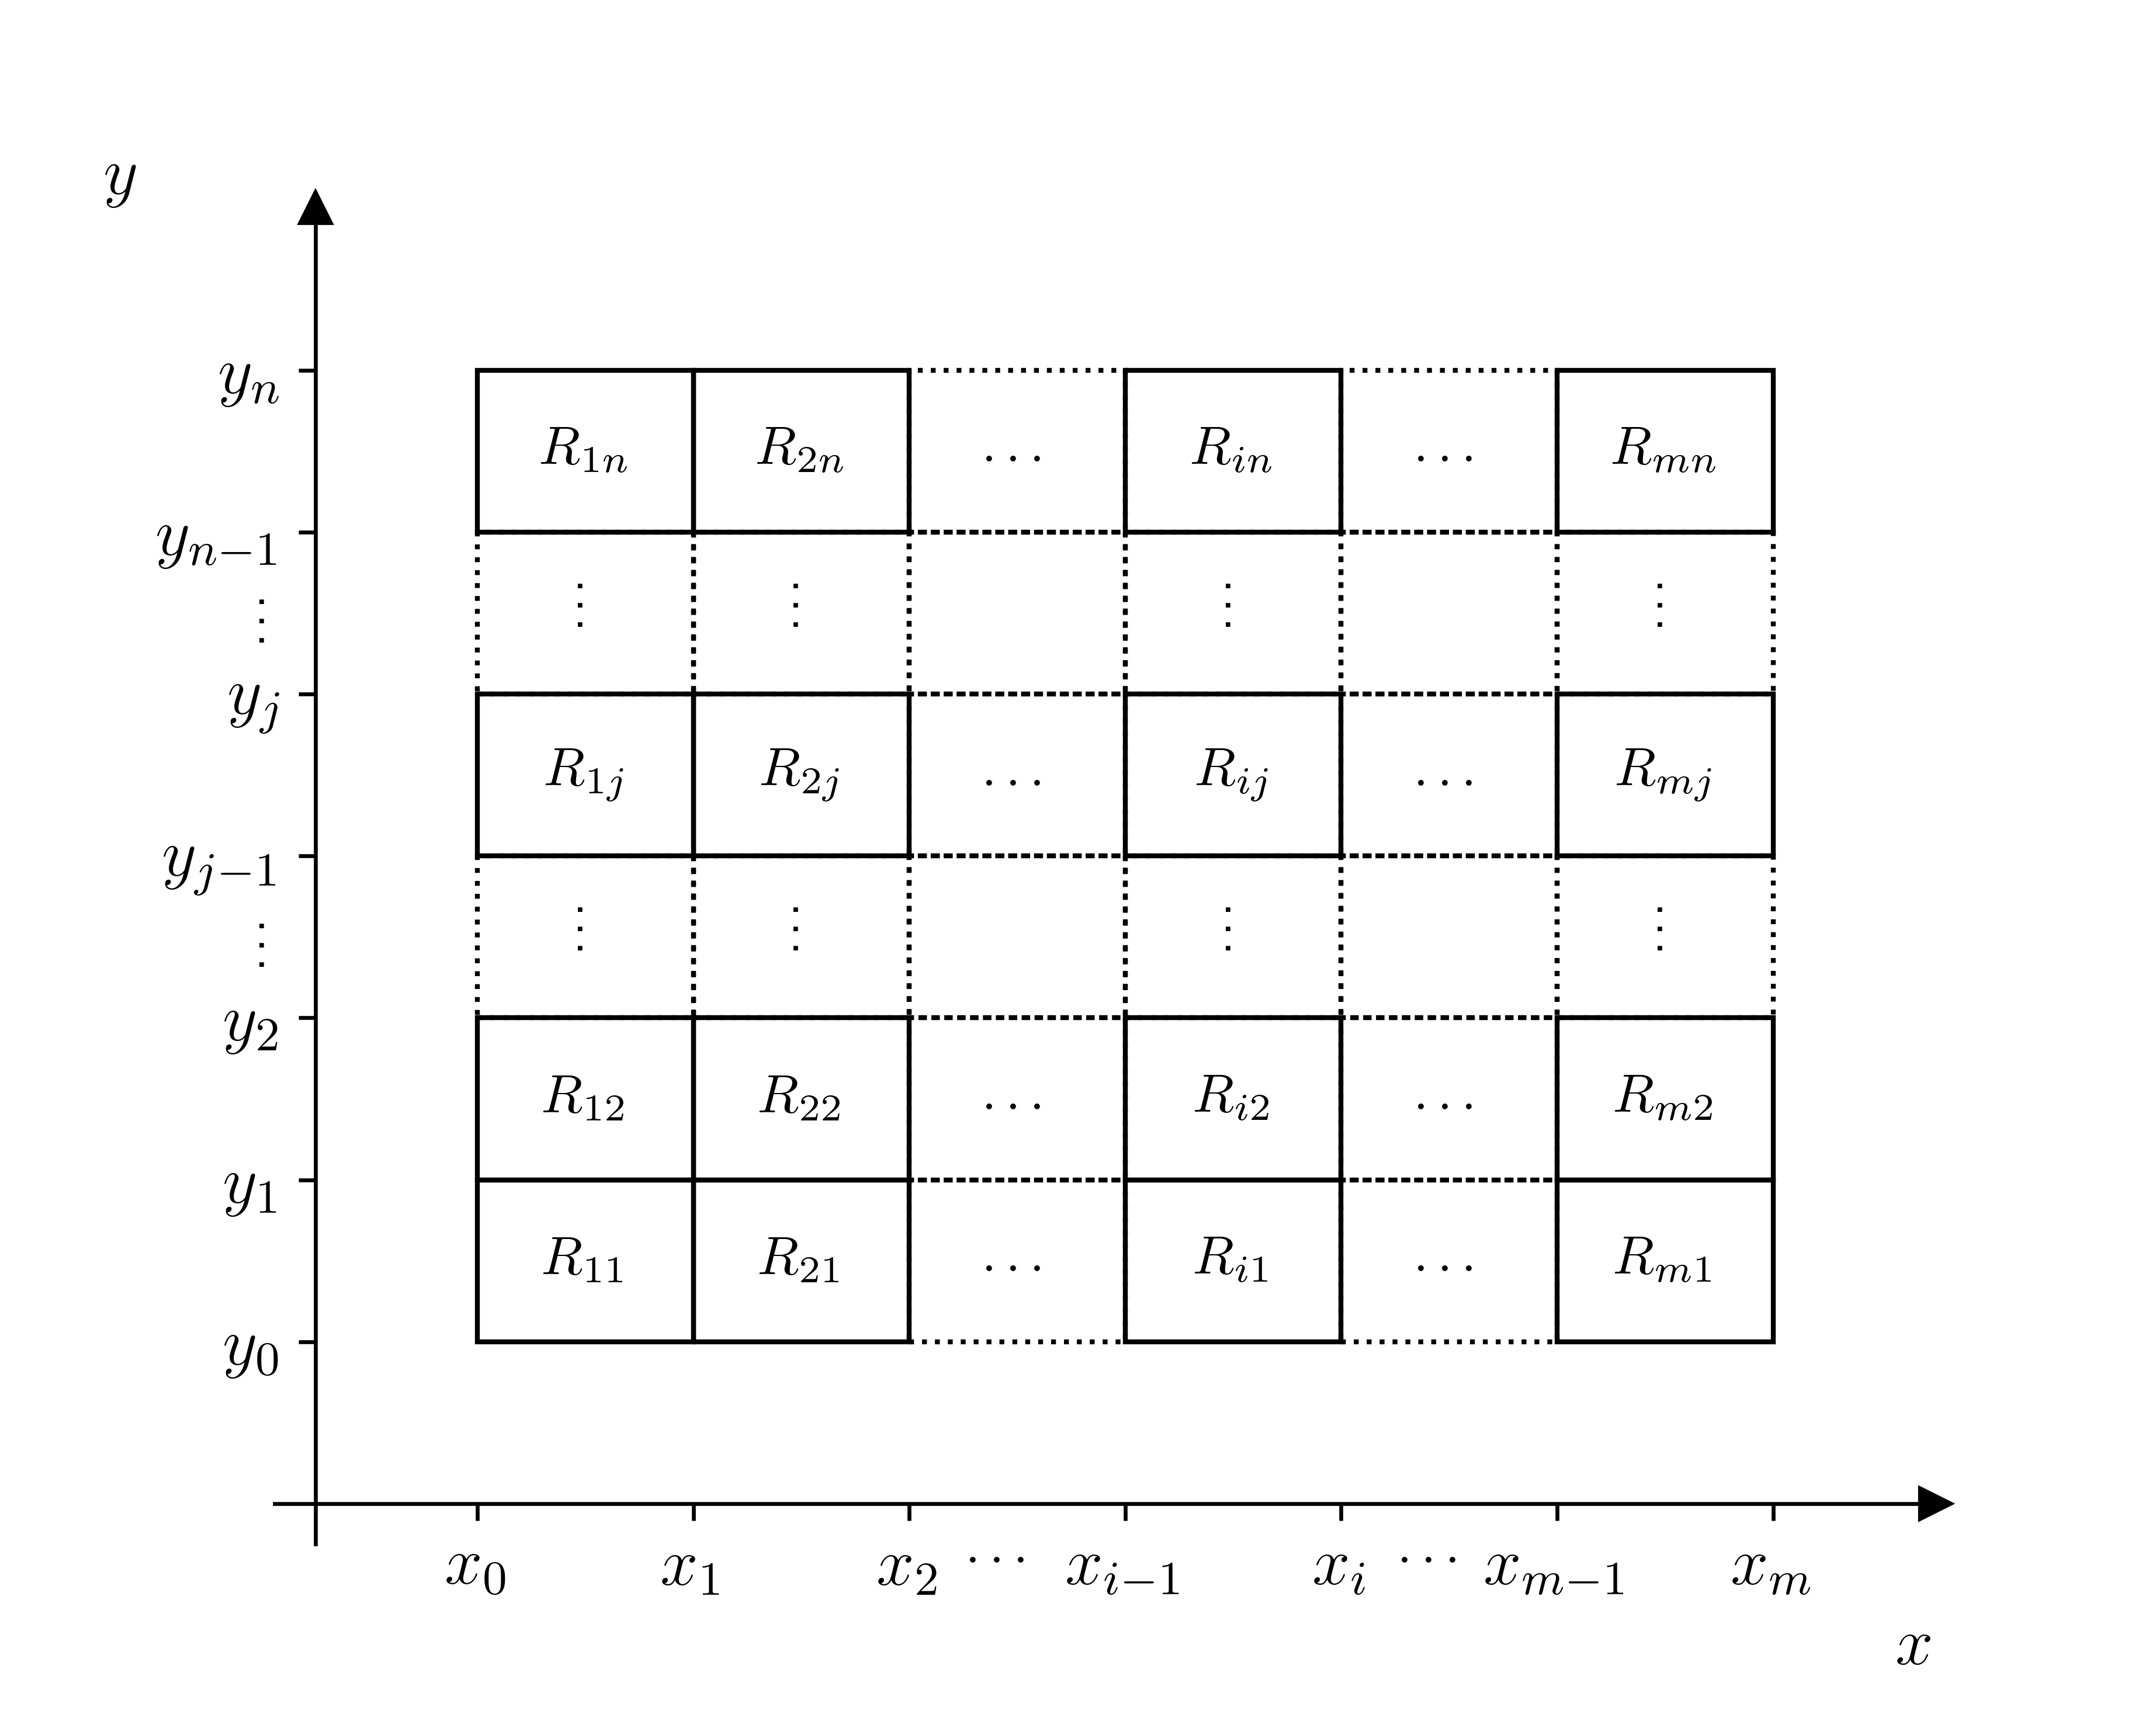
\includegraphics[scale=0.55]{./imagenes/Particion_Rectangulo.png}
  \caption{Partición de $R$}
\end{center}
\end{figure}
\end{frame}

\begin{frame}
  Sea $f:[a,b]\times[c,d]\To\Real$ una suma de Riemann es
  $$\sum_{i=1}^{m}\sum_{j=1}^{n}f(x_i^*,y_j^*)\Delta A_{ij}$$
  y
  $$\norm{P}=\max\set{\Delta A_{ij}}$$
  \onslide<2->{
  La integral doble en el rectángulo $R$ será
  $$\iint_R f(x,y)dA=\lim_{\norm{P}\to 0}\sum_{i=1}^{m}\sum_{j=1}^{n}f(x_i^*,y_j^*)\Delta A_{ij}$$
  Si dicho límite existe.}
\end{frame}

\begin{frame}
\begin{figure}[ht]
  \hspace*{-2.25cm}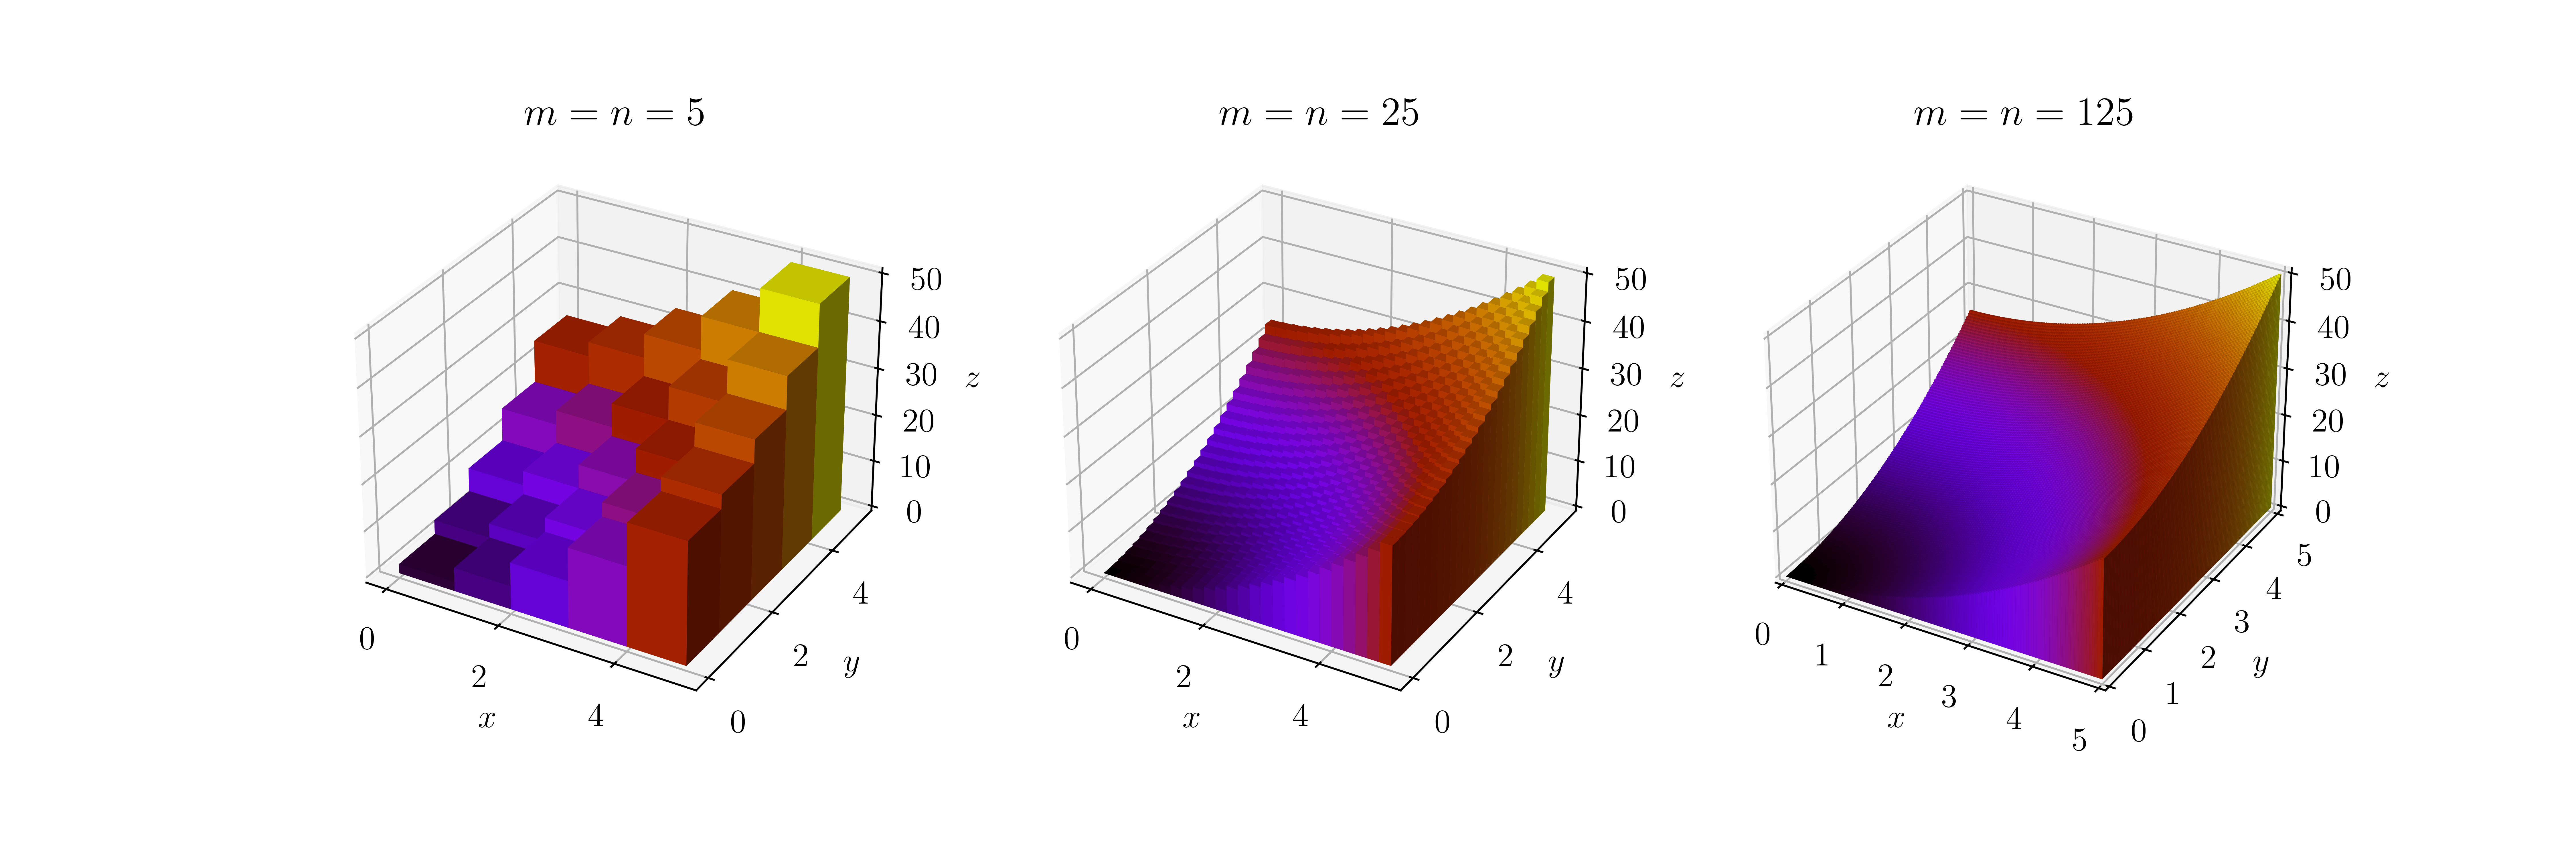
\includegraphics[scale=0.375]{./imagenes/Suma_Riemann3D_triple.png}
  \caption{Suma de Riemann $f(x,y) = x^2 + y^2$}
\end{figure}
\end{frame}

\begin{frame}{Ejemplos}
\begin{itemize}[<+->]
  \item Estime el volumen bajo la superficie dada por $f(x,y)=xy$ en $[0,6]\times[0,4]$ usando sumas de Riemann con $m=3$ y $n=2$
  \begin{itemize}
  \item usando el extremo superior derecho.
  \item usando el punto medio.
  \end{itemize}
  \item Se da la siguiente tabla de valores para una función $f(x,y)$ en $R=[1,3]\times[0,4]$
  \begin{center}
  \begin{tabular}{|c||c|c|c|c|c|c|c|}
  \hline
      & 0 & 1 & 2  & 3  & 4  \\
  \hline
  \hline
  1   & 2 & 0 & -3 & -6 & -5 \\
  \hline
  1,5 & 3 & 1 & -4 & -8 & -6 \\
  \hline
  2   & 4 & 3 & 0  & -5 & -8 \\
  \hline
  2,5 & 5 & 5 & 3  & -1 & -4 \\
  \hline
  3   & 7 & 8 & 6  & 3  & 0  \\
  \hline
  \end{tabular}
  \end{center}
  Estime $\int\!\!\!\int_R f(x,y)dA$
\end{itemize} 
\end{frame}

%! subsección
\subsection{Integrales Sobre Regiones Rectangulares}
\begin{frame}
\subsectionpage
\end{frame}

% \begin{frame}
% \tableofcontents[currentsubsection]
% \end{frame}

\begin{frame}
\begin{thm}
  Sea $f:\intervaloCC{a,b}\times \intervaloCC{c,d}\To\Real$ una función acotada que es continua salvo quizás en un conjunto que es unión finita de gráficas de funciones continuas de una variable, entonces f es integrable en $\intervaloCC{a,b}\times \intervaloCC{c,d}$.
\end{thm}
\end{frame}

\begin{frame}
\begin{block}{Teorema de Fubini}
  Sea $f:\intervaloCC{a,b}\times \intervaloCC{c,d}\To\Real$ una función acotada que es continua salvo quizás en un conjunto que es unión finita de gráficas de funciones continuas de una variable, si para todo $x\in\intervaloCC{a,b}$ la integral $\int_c^d f(x,y) dy$ existe, entonces $\int_a^b\int_c^d f(x,y) dydx$ existe y además
  $$\iint f(x,y) dA=\int_a^b\int_c^d f(x,y) dydx$$
  de manera similar si para todo $y\in\intervaloCC{c,d}$ la integral $\int_a^b f(x,y) dx$ existe, entonces $\int_c^d\int_a^b f(x,y) dxdy$ existe y además
  $$\iint f(x,y) dA=\int_c^d\int_a^b f(x,y) dxdy$$
\end{block}
\end{frame}

\begin{frame}
  \begin{prop}
  Sean $f,g:R=\intervaloCC{a,b}\times\intervaloCC{c,d}\To\Real$ funciones integrales, $\alpha,\beta\in\Real$
  \begin{enumerate}
    \item $\alpha f+\beta g$ es integrable en $R$ además
    $$\iint_R(\alpha f(x,y)+\beta g(x,y))dA=\alpha\iint_R f (x,y)dA+\beta\iint_R g(x,y)dA$$
    \item Si $R_1$ y $R_2$ son subrectángulos de $R$ tales que $R=R_1\bigcup R_2$ y $R_1$, $R_2$ comparten solo un borde entonces 
    $$\iint_{R_1\bigcup R_2} f(x,y)dA=\iint_{R_1} f(x,y)dA+\iint_{R_2} f(x,y)dA$$
    \item Si $f\geq 0$ en $R$ entonces $\iint_R f(x,y)dA\geq 0$
    \item Si $f\geq g$ en $R$ entonces $\iint_R f(x,y)dA\geq\iint_R g(x,y)dA$
  \end{enumerate}
  \end{prop}
\end{frame}

\begin{frame}{Ejemplos}
  Calcule las siguientes integrales en la región indicada
  \begin{enumerate}[<+->]
    \item $\displaystyle\iint_{R} x^2y+x^3+y^3 dA$, para $R=[1,2]\times[0,1]$
    \item $\displaystyle\iint_{R} (x^3-3x)\cos(2y) dA$, para $R=[0,1]\times[0,\frac{\pi}{2}] $
    % \item $\displaystyle\iint_R\,\left(sin(x)\left[\frac{x}{2}\right]+cos^2(y)+2\right)\,dA$, para $R=[0,5]\times[0,\pi]$.
  \end{enumerate}
\end{frame}  

%! subsección
\subsection{Integrales Sobre Regiones Generales}
\begin{frame}
\subsectionpage
\end{frame}

% \begin{frame}
% \tableofcontents[currentsubsection]
% \end{frame}

\begin{frame}
\begin{defn}
\begin{enumerate}[<+->]
  \item Diremos que una región $D\subseteq\Real^2$ es elemental de primer tipo si existen funciones continuas $\psi_1,\psi_2:\intervaloCC{a,b}\To\Real$ tales que para todo $x\in\intervaloCC{a,b}$ $\psi_1(x)\leq\psi_2(x)$ y
  $$D=\set{(x,y)\in\Real^2\ :\ a\leq x\leq b\wedge\psi_1(x)\leq y\leq\psi_2(x)}$$
  \item Diremos que una región $D\subseteq\Real^2$ es elemental de segundo tipo si existen funciones continuas $\phi_1,\phi_2:\intervaloCC{c,d}\To\Real$ tales que para todo  $y\in\intervaloCC{c,d}$ $\phi_1(y)\leq\psi_2(y)$ y
  $$D=\set{(x,y)\in\Real^2\ :\ c\leq y\leq d\wedge\phi_1(y)\leq x\leq\phi_2(y)}$$
\end{enumerate}
\end{defn}
\end{frame}

\begin{frame}
\begin{figure}
\begin{center}
  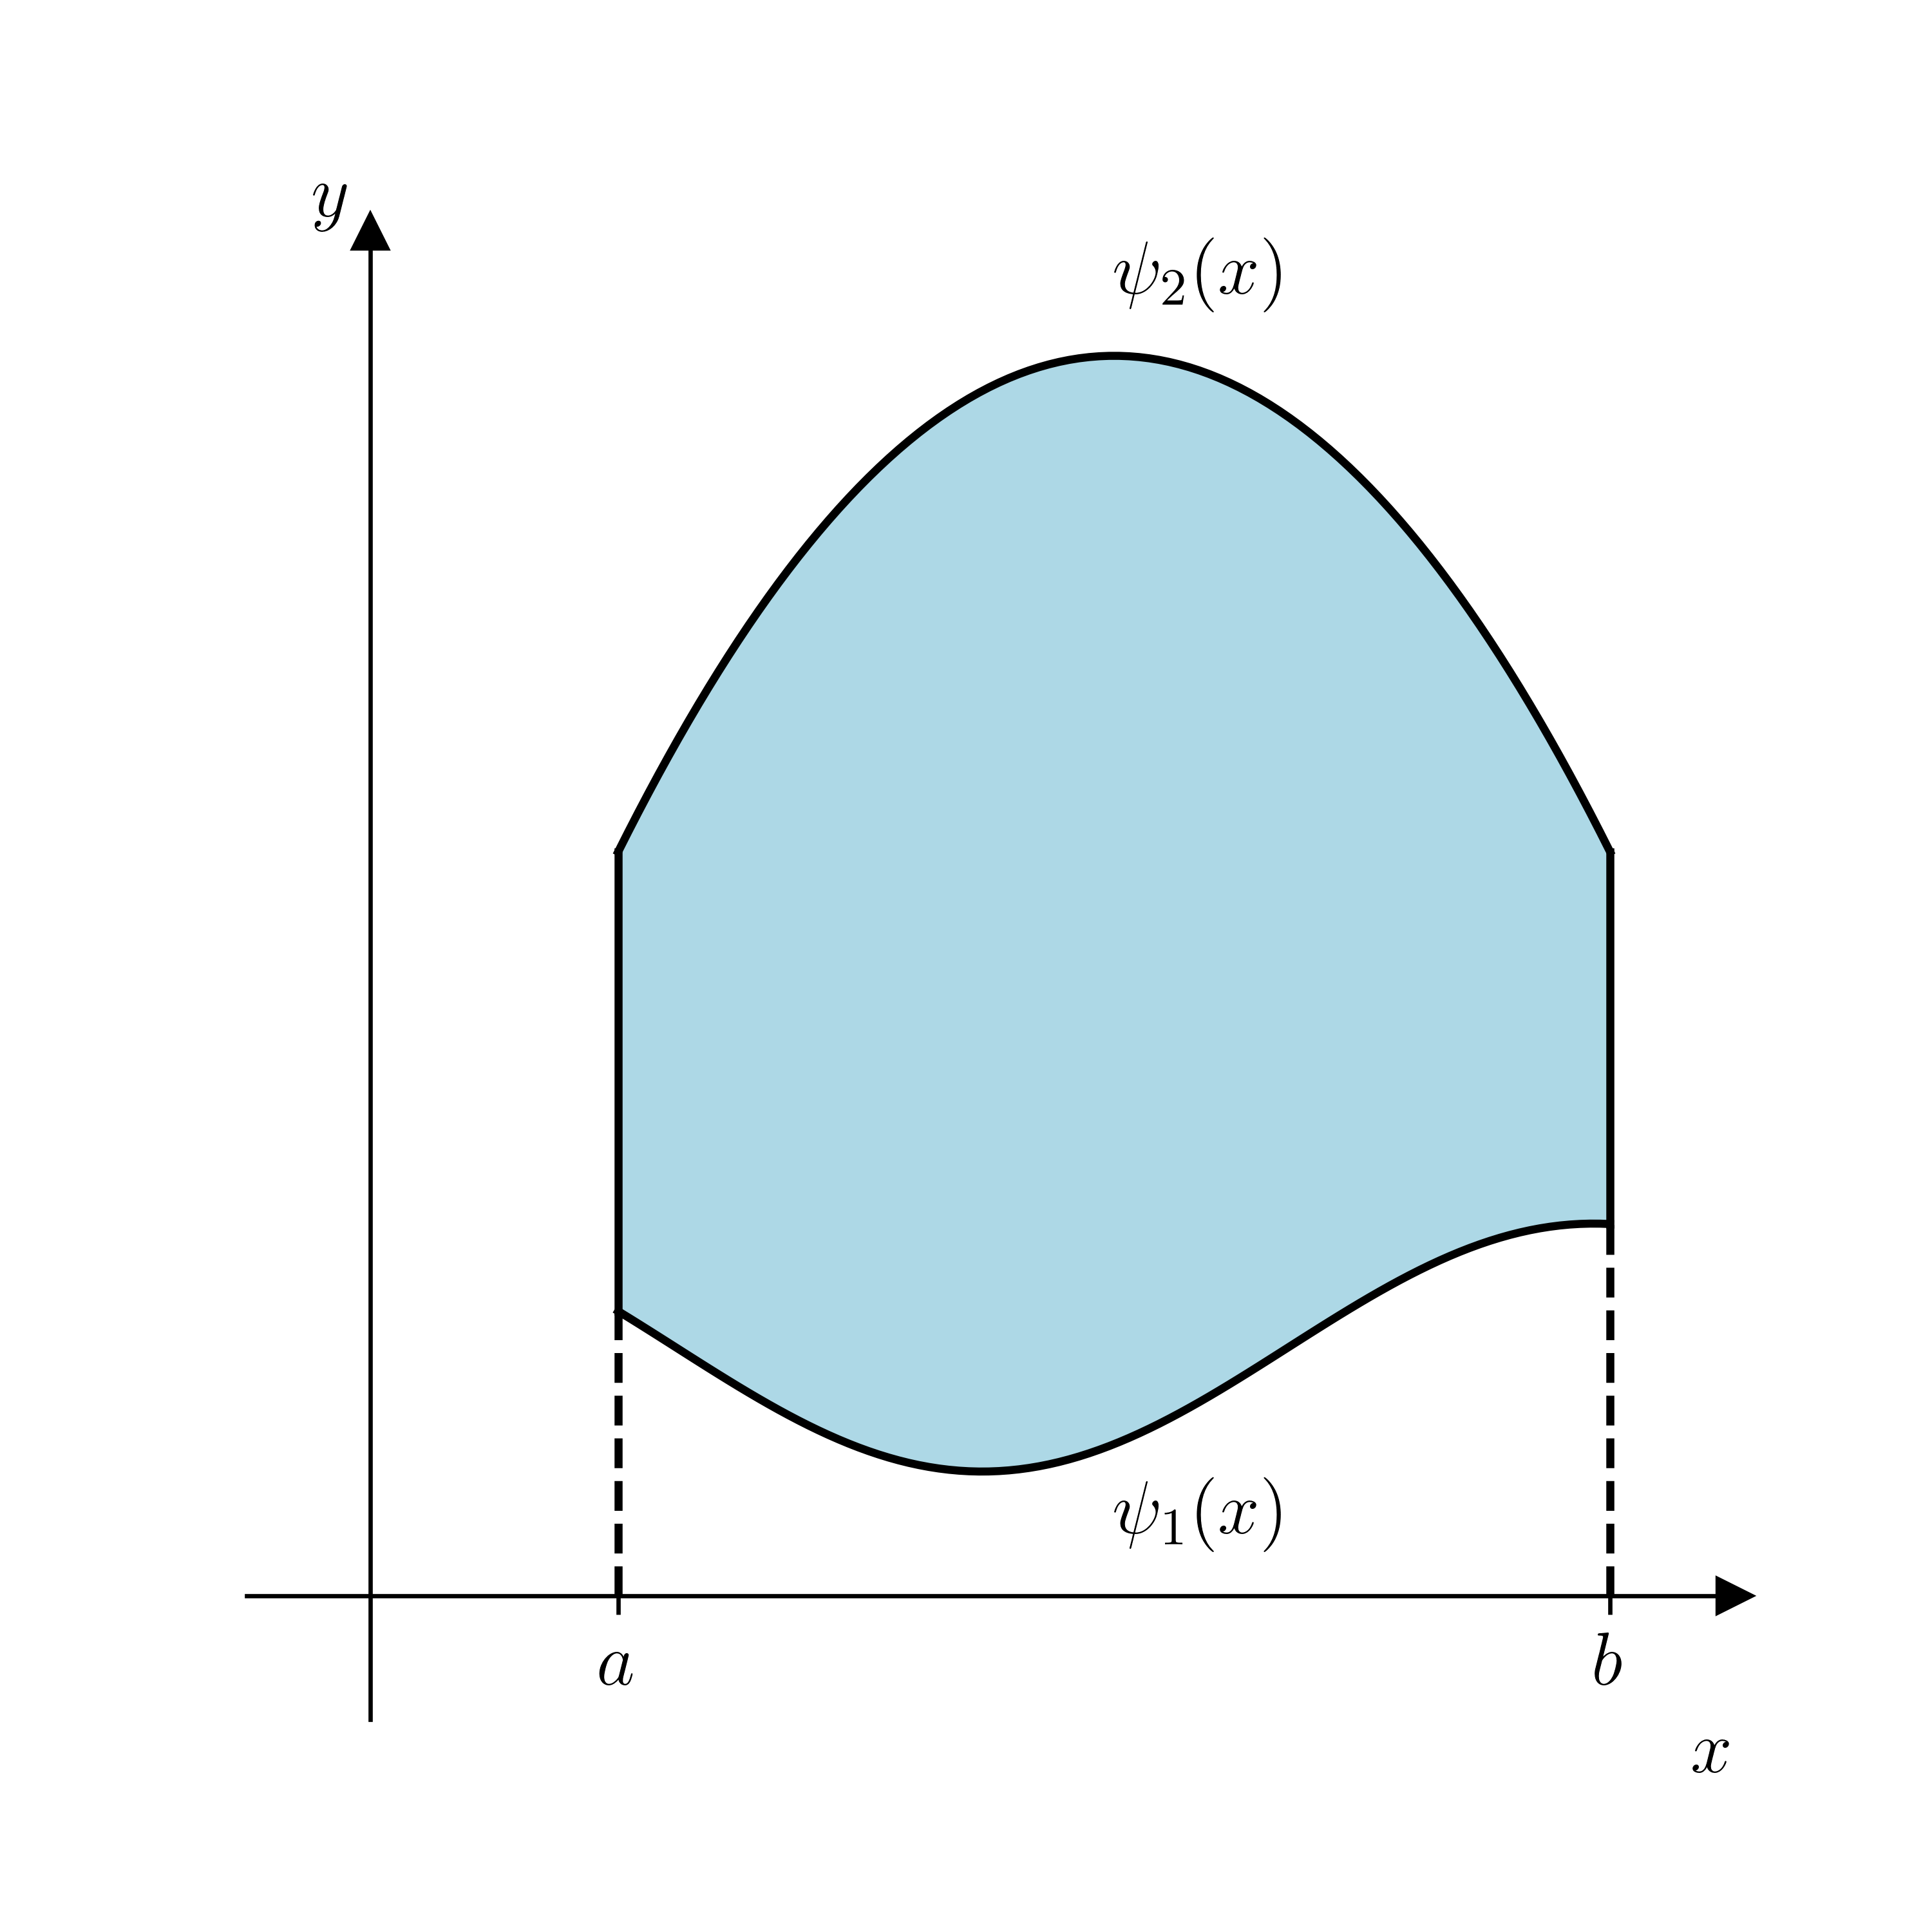
\includegraphics[scale=0.6]{./imagenes/Region_Tipo1.png}
  \vspace{-5mm}
  \caption{Region de primer tipo}
\end{center}
\end{figure}
\end{frame}

\begin{frame}
  \begin{thm}
    Sea $f:D\subseteq\Real^2\To\Real$ una función continua en $D$.
    \begin{enumerate}[<+->]
      \item Si $D$ es una región elemental de primer tipo, entonces
      $$\iint_D f(x,y)dA=\int_a^b\int_{\psi_1(x)}^{\psi_2(x)}f(x,y)\ dydx$$
      \item Si $D$ es una región elemental de segundo tipo, entonces
      $$\iint_D f(x,y)dA=\int_c^d\int_{\phi_1(y)}^{\phi_2(y)}f(x,y)\ dxdy$$
    \end{enumerate}
  \end{thm}
\end{frame}

\begin{frame}
\begin{rem}
  El area de una región elemental $D$ se puede calcular como
  $$\iint_D 1 dA$$
\end{rem}
\end{frame}

\begin{frame}{Ejemplos}
  Calcule las siguientes integrales en la región indicada\\[0.5cm]
  \begin{enumerate}[<+->]
    \item $\displaystyle\iint_{R} e^{y^2} dA$, para $R=\set{(x,y):0\leq x\leq 1\wedge x\leq y\leq 1}$\\[0.25cm]
    % \item $\displaystyle\iint_{R} \frac{\sen(x)}{x} dA$, $R$ el triangulo de vertices $(0,0)$, $(0,1)$ y $(1,1)$\\[0.25cm]
    \item Calcule el área de la región
    $$\Omega=\{(x,y)\in\Real^2\,:\,0\leq y \leq 2, \: y-1 \leq x \leq e^y\}.$$
    % \item Calcule el volumen del solido limitado superiormente por la gráfica de la función $f(x,y)=1-|x|-|y|$, e inferiormente por el plano $z=0$.
  \end{enumerate}
\end{frame}

%! subsección
\subsection{Cambio de Variables en Integrales Dobles}
\begin{frame}
\subsectionpage
\end{frame}

% \begin{frame}
% \tableofcontents[currentsubsection]
% \end{frame}

\begin{frame}
\begin{thm}
  Sean $D$ y $D^*$ regiones elementales en el plano. Sea 
  $$\begin{array}{rrcl}
    F:&D^*  &\to    & D\\
      &(u,v)&\mapsto& (x(u,v),y(u,v))
  \end{array}$$
  $C^1$ y biyectiva, si $f:D\to\Real$ es integrable, entonces
  $$\iint_D f(x,y) dxdy=\iint_{D^*} f(x(u,v),y(u,v))\abs{J} dudv$$
  donde
  %! volví a la notación tradicional pues es la que aparece en los libros guía
  $$J=\frac{\delta(x,y)}{\delta(u,v)}=\det(D_{(u,v)}(x,y))=\det\left(\begin{array}{rr}
    \frac{\delta x}{\delta u} & \frac{\delta x}{\delta v}\\
    \frac{\delta y}{\delta u} & \frac{\delta y}{\delta v}\\
  \end{array}\right)$$
  es llamado {\bf Jacobiano} (el determinante de la matriz jacobiana $D_{(u,v)}(x,y)$).
\end{thm}
\end{frame}

\begin{frame}
\begin{block}{Integrales dobles en coordenadas polares}
  Dada una region $D$ que se puede expresar como una región elemental $D^*$ en coordenadas polares.
  $$\iint_D f(x,y) dxdy=\iint_{D^*} f(r\cos(\theta),r\sen(\theta))r\ drd\theta$$
\end{block}
\end{frame}

\begin{frame}{Ejemplos}
  Calcule las siguientes integrales usando un cambio de variable conveniente
  \begin{enumerate}[<+->]
    \item $\displaystyle\iint_{D} x+y dA$, donde $D$ es la región del primer cuadrante acotada por las circunferencias $x^2+y^2=1$ y $x^2+y^2=4$.
    \item $\displaystyle\iint_{D} 1+x+y dA$, donde $D$ es la región acotada por las rectas $y-x=1$, $y-x=-1$, $y+x=1$, $y+x=2$.
    % \item $\displaystyle\iint_{D} x^2y^2 dA$, donde $D$ es la región acotada por las curvas $xy=1$, $xy=2$, $y=\frac{x}{2}$ , $y=3x$.
  \end{enumerate}
\end{frame}

%! subsección
\subsection{Ejercicios}
\begin{frame}
\subsectionpage
\end{frame}

% \begin{frame}
% \tableofcontents[currentsubsection]
% \end{frame}

\begin{frame}{Ejercicios}
  \vspace{-5mm}
  \begin{enumerate}
    \item Se da la siguiente tabla de valores para una función $f(x,y)$ en $R=[1,3]\times[1,4]$
      \begin{center}
      \begin{tabular}{|c||r|r|r|r|}
      \hline
          & 1 &  2 &  3 &  4 \\
      \hline
      \hline
      1   & 0 & -1 & -2 & -2 \\
      \hline
      2   & 3 &  0 & -1 &  1 \\
      \hline
      3   & 5 &  3 &  2 &  0 \\
      \hline
      \end{tabular}
      \end{center}
    Estime $\int\!\!\!\int_R f(x,y)dA$
    \vspace{3mm}
    \item Calcule las siguientes integrales.
      \begin{enumerate}
        \item $\displaystyle\iint_{R} x^3+x^2y^2+x^2+y^2 dA$, para $R=[1,2]\times[0,1]$
        \item $\displaystyle\iint_{R} 4xe^{2y+x^2} dA$, para $R=[0,1]\times[1,2] $
      \end{enumerate}
  \end{enumerate}
\end{frame}

\begin{frame}{Ejercicios}
  \vspace{-5mm}
  \begin{enumerate}
    \setcounter{enumi}{2}
    %\item Sea $D=\{(x,y)\in \Real^2: 0\leq x\leq 2\,\,\wedge\,\, x\leq y\leq 2x\}$ y sea $f$ una función integrable sobre la región $D$. Cambia el orden de integración para la siguiente integral
    \item Cambie el orden de integración para la siguiente integral.
    $$\int_0^2\int_{x}^{2x}f(x,y)\,\mathrm{d}y\,\mathrm{d}x. $$
    \item  Calcule, si es posible, el valor de
    \vspace{-1mm}
    $$\int_{1}^2\, \int_0^{\ln x}(x-1)\sqrt{1+e^{2y}}\,\mathrm{d}y\,\mathrm{d}x.$$
    \item Sea $D=\{(x,y)\in\Real^2: 0\leq x\leq 1\,\,\wedge\,\, 0\leq y\leq 2\}$ y %sea  $f:D\rightarrow \Real$ la función definida por
    % $$f(x,y)= \left\{\begin{array}[c]{lll}
    % 1+x& \mbox{si } (x,y)\in D_1=\{(x,y)\in D: x>2y\} \medskip\\
    % -1-y& \mbox{si } (x,y)\in D_2=\{(x,y)\in D: x\leq 2y\} .
    % \end{array}\right.$$
    $$f(x,y)=\begin{cases}
      1+x  & \text{si } (x,y)\in D_1\\
      -1-y & \text{si } (x,y)\in D_2
    \end{cases}$$
    con $D_1=\{(x,y)\in D: x>2y\}$, $D_2=\{(x,y)\in D: x\leq 2y\}$, halle el volumen del sólido limitado por la superficie $z=f(x,y)$ y el plano $xy$, con $(x,y)\in D$.
  \end{enumerate}
\end{frame}

\begin{frame}{Ejercicios}
  \begin{enumerate}
    \setcounter{enumi}{5}
    \item Calcule las siguientes integrales usando un cambio de variable conveniente
      \begin{enumerate}
        \item $\displaystyle\iint_{D} x^2y dA$, donde $D$ es la mitad superior del disco  con centro en el origen y radio 5.
        \item $\displaystyle\iint_{D} e^{-x^2-y^2} dA$, donde $D$ es la región en el primer cuadrante entre las circunferencias con centro en el origen y radios 1 y 3.
        % \item determine el área de la región $D$ en el primer cuadrante acotada por las curvas $y=x^2$, $y=2x^2$, $x=y^2$, $x=4y^2$
        \item $\displaystyle\iint_{D} e^{-\sqrt{\frac{x^2}{4}+\frac{y^2}{9}}} dA$, donde $D=\set{(x,y)\in\Real^2\ :\ \frac{x^2}{4}+\frac{y^2}{9}\leq 1}$.
      \end{enumerate}
  \end{enumerate}
\end{frame}

%! sección
\section{Integrales Triples}
\begin{frame}
\sectionpage
\end{frame}

\begin{frame}
\tableofcontents[currentsection]
\end{frame}

%! subsección
\subsection{Integrales Triples}
\begin{frame}
\subsectionpage
\end{frame}

% \begin{frame}
% \tableofcontents[currentsubsection]
% \end{frame}

\begin{frame}
  En integrales triples se satisface el equivalente al teorema de Fubini que vimos en integrales dobles y para condiciones análogas tendremos
  \begin{eqnarray*}
    \iiint_{\intervaloCC{a,b} \times \intervaloCC{c,d} \times \intervaloCC{p,q}}f\left( x,y,z\right) \mathrm{d}V
    &=&\int_a^b\int_c^d\int_p^q f(x,y,z) dz dy dx\\
    &=&\int_c^d\int_a^b\int_p^q f(x,y,z) dz dx dy\\
    &=&\cdots
  \end{eqnarray*}
\end{frame}

\begin{frame}{Ejemplo}
  Calcule
  $$\iiint_{\intervaloCC{0,1} \times \intervaloCC{1,2} \times \intervaloCC{-1,1}
  }\left( x^{2}y+zy^{2}\right) \mathrm{d}\left( x,y,z\right)$$
\end{frame}

\begin{frame}
  Para las integrales triples, las regiones elementales son como 
  \begin{defn}
  Una región elemental respecto al plano $xy\,$\ es una región de la forma
  \onslide<2->{
  \begin{equation*}
  T=\left\{ \left( x,y,z\right) \in \mathbb{R}^{3}:\left( x,y\right) \in
  R,k_{1}\left( x,y\right) \leq z\leq k_{2}\left( x,y\right) \right\}
  \end{equation*}
  }
  \onslide<3->{
  donde $R$ es una región elemental en $\mathbb{R}^{2}$ y $k_{1}\left(
  x,y\right) ,k_{2}\left( x,y\right) $ son funciones continuas en $R$.
  }
  \end{defn}
\end{frame}

\begin{frame}
  \begin{center}
  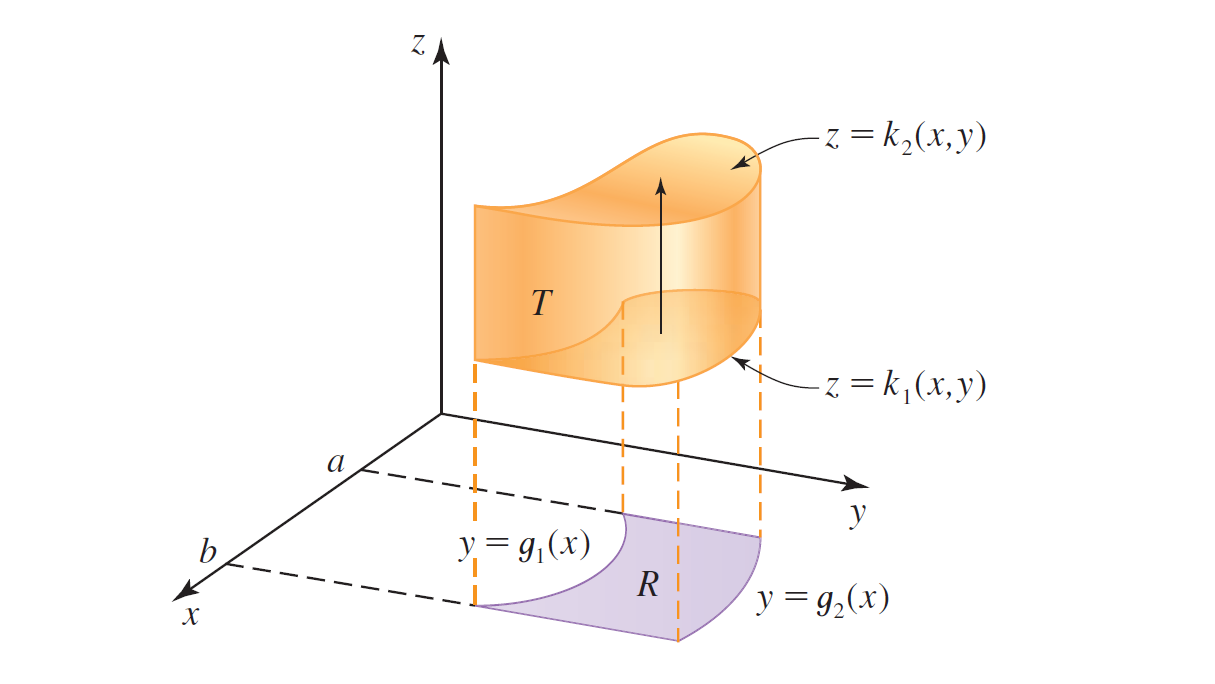
\includegraphics[scale=0.2]{./imagenes/Clases1-Elemental3D-1.png}
  \end{center}
  En la figura vemos una región elemental respecto al plano $xy$ en este caso
  la integral triple quedaría
  \onslide<2->{
  \begin{eqnarray*}
  \iiint_{T}f\left( x,y,z\right) \mathrm{d}V &=&\iint_{R}\int_{k_{1}\left(
  x,y\right) }^{k_{2}\left( x,y\right) }f\left( x,y,z\right) \mathrm{d}z%
  \mathrm{d}A \\
  \onslide<3->{
  &=&\int_{a}^{b}\int_{g_{1}\left( x\right) }^{g_{2}\left( x\right)
  }\int_{k_{1}\left( x,y\right) }^{k_{2}\left( x,y\right) }f\left(
  x,y,z\right) \mathrm{d}z\mathrm{d}y\mathrm{d}x
  }
  \end{eqnarray*}
  }
\end{frame}

\begin{frame}
  \begin{egs}
    \begin{enumerate}
      \item Escribir distintas formas de calcular
      \begin{equation*}
      \iiint_{T}f\left( x,y,z\right) \mathrm{d}V
      \end{equation*}
      donde
      \begin{equation*}
      T=\left\{ \left( x,y,z\right) \in \mathbb{R}^{3}:\frac{x^{2}}{4}+y^{2}+\frac{z^{2}}{9}\leq 1\right\}
      \end{equation*}
      \item<2-> Calcular
      \begin{equation*}
      \iiint_{T}\sqrt{x^{2}+z^{2}}\mathrm{d}V
      \end{equation*}
      donde $T$ es la región acotada por el cilindro $x^{2}+z^{2}=1$ y los planos $y+z=2$, $y=0$.
    \end{enumerate}
  \end{egs}
\end{frame}

%! subsección
\subsection{Cambio de Variables en Integrales Triples}
\begin{frame}
\subsectionpage
\end{frame}

% \begin{frame}
% \tableofcontents[currentsubsection]
% \end{frame}

\begin{frame}
  \begin{thm}
  Sean $D$ y $D^*$ regiones elementales en el espacio. Sea 
  $$\begin{array}{rrcl}
  F:&D^*  &\to    & D\\
    &(u,v,w)&\mapsto& (x(u,v,w),y(u,v,w),z(u,v,w))
  \end{array}$$
  $C^1$ y biyectiva, si $f:D\to\Real$ es integrable, entonces\\
  \vspace{5mm}
  \resizebox*{\textwidth}{!}{
    $\displaystyle\iiint_D f(x,y) d(x,y,z)=\iiint_{D^*} f(x(u,v,w),y(u,v,w),z(u,v,w))\abs{J} d(u,v,w)$
  }\\
  \vspace{5mm}
  donde
  %! volví a la notación tradicional pues es la que aparece en los libros guía
  $$J=\frac{\delta(x,y,z)}{\delta(u,v,w)} = 
    \det\left(\left[\begin{array}{rrr}
    \frac{\delta x}{\delta u} & \frac{\delta x}{\delta v} & \frac{\delta x}{\delta w}\\
    \frac{\delta y}{\delta u} & \frac{\delta y}{\delta v} & \frac{\delta y}{\delta w}\\
    \frac{\delta z}{\delta u} & \frac{\delta z}{\delta v} & \frac{\delta z}{\delta w}
  \end{array}\right]\right)$$
  es el determinante de la {\bf Matriz Jacobiana} correspondiente.
  \end{thm}
\end{frame}

\begin{frame}
  \begin{eg}
    Resuelva la siguiente integral
    $$\iiint_{\Omega}\,(4x-3y-5z)\,dV$$
    \noindent donde $\Omega$ es el conjunto acotado entre los planos
    $$\left\{\begin{array}{l}
      \Pi_1\,=\,5x-2y+4z=2\\
      \Pi_2\,=\,5x-2y+4z=5\\
      \Pi_3\,=\,-3x-2y-4z=0\\
      \Pi_4\,=\,-3x-2y-4z=5\\
      \Pi_5\,=\,2x+y-5z=0\\
      \Pi_6\,=\,2x+y-5z=4\\
    \end{array}\right.$$
  \end{eg}
\end{frame}

\begin{frame}{Coordenadas Cilindricas}
  \vspace{-5mm}
  El cambio de variables dado por 
  \begin{eqnarray*}
    x &=& r\cos(\theta)\\
    y &=& r\sen(\theta)\\
    z &=& z
  \end{eqnarray*}
  con $r\geq 0$ y $\theta\in[0,2\pi]$ es interpretado como describir los puntos en coordenadas cilíndricas.\\
  \begin{figure}
    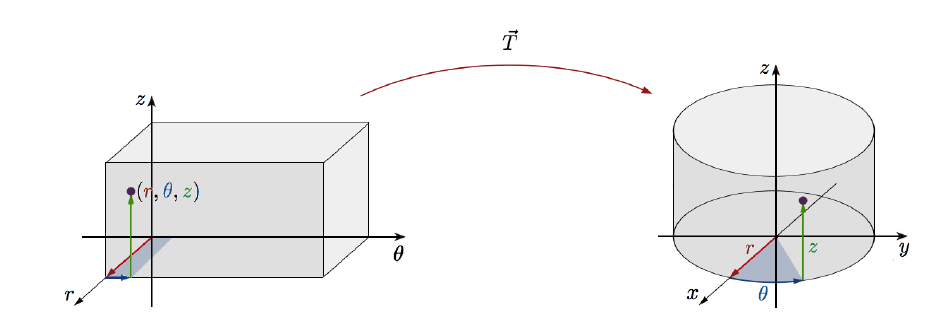
\includegraphics[scale=0.3]{./imagenes/Clases1-Cilindricas.png}
  \end{figure}
\end{frame}

\begin{frame}{Coordenadas Cilindricas}
  \begin{thm}
    Si una región $D$ se puede expresar como la región elemental $D^*$ en coordenadas cilíndricas, entonces
    $$\iiint_D f(x,y,z) d(x,y,z)=\iiint_{D^*} f(r\cos(\theta),r\sen(\theta),z)\ r\ d(r,\theta,z)$$
  \end{thm}
  \onslide<2->{
  \begin{eg}
    Calcule el volumen del sólido encerrado por la esfera $x^2+y^2+z^2=16$ y el cilindro $(x-2)^2+y^2=4$.
  \end{eg}
  }
\end{frame}

\begin{frame}{Coordenadas Esfericas}
  \vspace{-5mm}
  El cambio de variables dado por 
  \begin{eqnarray*}
    x &=& \rho\cos(\theta)\sen(\phi)\\
    y &=& \rho\sen(\theta)\sen(\phi)\\
    z &=& \rho\cos(\phi)
  \end{eqnarray*}
  $\rho\geq 0$, $\theta\in[0,2\pi]$ y $\phi\in[0,\pi]$ es interpretado como describir los puntos en coordenadas esféricas.\\
  \begin{figure}
    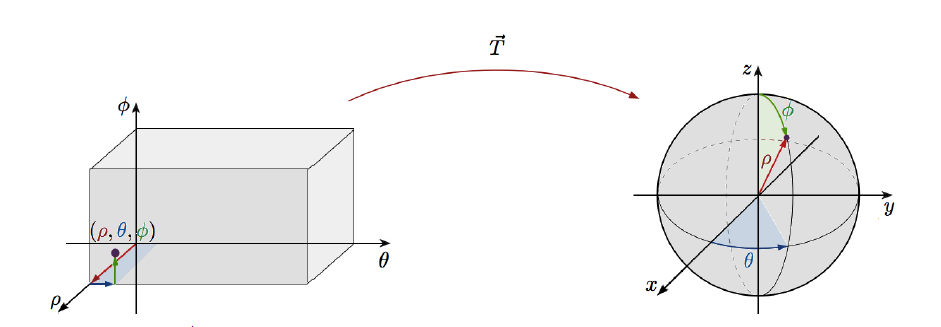
\includegraphics[scale=0.3]{./imagenes/Clases1-Esfericas.png}
  \end{figure}
\end{frame}

\begin{frame}{Coordenadas Esfericas}
  \vspace{-5mm}
  \begin{thm}
    Si una región $D$ se puede expresar como la región elemental $D^*$ en coordenadas esféricas, entonces.\\
    \vspace{5mm}
    \resizebox*{\textwidth}{!}{
      $\displaystyle\iiint_D f(x,y,z) d(x,y,z)=\iiint_{D^*} f(\rho\cos(\theta)\sen(\phi),\rho\sen(\theta)\sen(\phi),\rho\cos(\phi))\ \rho^2\sen(\phi) \ d(\rho,\theta,\phi)$
    }
  \end{thm}
  \onslide<2->{
  \begin{eg}
    Calcule el volumen del sólido encerrado por la esfera $x^2+y^2+z^2=4z$ y el cono $x^2+y^2=z^2$, contenido en la región $z\geq 0$.
  \end{eg}
  }
\end{frame}

%! subsección
\subsection{Ejercicios}
\begin{frame}
\subsectionpage
\end{frame}

% \begin{frame}
% \tableofcontents[currentsubsection]
% \end{frame}

\begin{frame}{Ejercicios}
  \begin{enumerate}
    \item Evalúe las siguientes integrales triples
    \begin{enumerate}
      \item $\displaystyle\iiint_{T} x^2+yz-y^2\ dV$, donde $T=[0,1]\times[0,3]\times[1,2]$.\\[0.25cm]
      \item $\displaystyle\iiint_{E} y\ dV$, donde 
      \scalebox{0.9}{$E=~\set{(x,y,z)\in\Real^3\ :\ 0\leq x\leq 3\ \wedge\ 0\leq y\leq x\ \wedge\ x-y\leq z\leq x+y}$}.\\[0.25cm]
      % $$E=~\set{(x,y,z)\in\Real^3\ :\ 0\leq x\leq 3\ \wedge\ 0\leq y\leq x\ \wedge\ x-y\leq z\leq x+y}$$
      \item $\displaystyle\iiint_{T} x^2+y^2+z^2\ dV$, donde $T$ es el conjunto acotado por el cilindro $x^2+y^2=1$ y los planos $z=0$ y $z=1$.\\[0.25cm]
      \item $\displaystyle\iiint_{E} x^2+y^2\ dV$, donde $E$ es la región entre las esferas $x^2+y^2+z^2=4$ y $x^2+y^2+z^2=9$. 
    \end{enumerate}
  \end{enumerate}
\end{frame}


% %! sección
% \section{Aplicaciones}
% \begin{frame}
% \sectionpage
% \end{frame}

% \begin{frame}
% \tableofcontents[currentsection]
% \end{frame}

% %! subsección
% \subsection{Aplicaciones de la Integral Doble}
% \begin{frame}
% \subsectionpage
% \end{frame}

% % \begin{frame}
% % \tableofcontents[currentsubsection]
% % \end{frame}

% \begin{frame}
% \begin{defn}
%   Consideremos una región $R\subseteq\Real^2$ y una función de densidad de masa $\rho:R\to\Real^+_0$, la masa total de la región será
%   $$M=\iint_R\ \rho(x,y) dA$$
%   \onslide<2->{
%   los primeros momentos están dados por
%   $$M_x=\iint_R\ y\rho(x,y) dA$$
%   $$M_y=\iint_R\ x\rho(x,y) dA$$
%   }
%   \onslide<3->{
%   y el centro de masa tendrá coordenadas
%   $$\bar{x}=\frac{M_y}{M},\ \ \bar{y}=\frac{M_x}{M}$$
%   }
% \end{defn}
% \end{frame}

% \begin{frame}
% \begin{defn}
%   Consideremos una región $R\subseteq\Real^2$ y una función de densidad de masa $\rho:R\to\Real^+_0$, los segundos momentos o mementos de inercia están dados por
%   \vspace{-3mm}
%   $$I_x=\iint_R\ y^2\rho(x,y) dA$$
%   $$I_y=\iint_R\ x^2\rho(x,y) dA$$
%   $$I_0=\iint_R\ (x^2+y^2)\rho(x,y) dA$$
%   $$I_L=\iint_R(r(x,y))^2 \,\rho(x,y) dA$$
%   donde $r(x,y)$ es la distancia  del punto $(x,y)$ a la recta $L$.\\
%   \onslide<2->{
%   \par Los radios de giro
%   \vspace{-3mm}
%   $$R_x=\sqrt{\frac{I_x}{M}},\ \ R_y=\sqrt{\frac{I_y}{M}}\text{ y }R_0=\sqrt{\frac{I_0}{M}}$$
%   }
% \end{defn}
% \end{frame}

% \begin{frame}{Ejemplos}
% \begin{enumerate}[<+->]
%   \item Calcule la masa de una lamina que corresponde a la región delimitada por la curva $\sqrt{1-x^2}$ y el semiplano $y\geq 0$ cuya densidad es $\rho=e^{x^2+y^2}$.\\
%   \vspace{5mm}
%   \item Determina el centroide de la región infinita ubicada en el segundo cuadrante y
%   comprendida entre los ejes coordenados y la curva $y=e^x$.\\
%   \vspace{5mm}
%   \item Determine el momento de inercia con respecto del eje $Y$, de la región triangular de vértices $A=(1,1)$, $B=(3,1)$ y $C=(3,5)$, si la densidad de área de la región esta dada por $\rho(x,y)=x+y$.
% \end{enumerate}
% \end{frame}

% %! subsección
% \subsection{Aplicaciones de la Integral Triple}
% \begin{frame}
% \subsectionpage
% \end{frame}

% % \begin{frame}
% % \tableofcontents[currentsubsection]
% % \end{frame}

% \begin{frame}
%   \begin{defn}
%     Consideremos una región $R\subseteq\Real^3$ y una función de densidad de masa $\rho:R\to\Real^+_0$, la masa total de la región será
%     \vspace{-3mm}
%     $$M=\iiint_R\ \rho(x,y,z) dV$$
%     \onslide<2->{
%     los primeros momentos están dados por
%     \vspace{-3mm}
%     $$M_{yz}=\iiint_R\ x\rho(x,y,z) dV$$
%     $$M_{xz}=\iiint_R\ y\rho(x,y,z) dV$$
%     $$M_{xy}=\iiint_R\ z\rho(x,y,z) dV$$
%     }
%     \onslide<3->{
%     y el centro de masa tendrá coordenadas
%     \vspace{-3mm}
%     $$\bar{x}=\frac{M_{yz}}{M},\ \ \bar{y}=\frac{M_{xz}}{M},\ \ \bar{z}=\frac{M_{xy}}{M}$$
%     }
%   \end{defn}
% \end{frame}

% \begin{frame}
%   \begin{defn}
%     Consideremos una región $R\subseteq\Real^3$ y una función de densidad de masa $\rho:R\to\Real^+_0$, los segundos momentos o mementos de inercia están dados por
%     \vspace{-3mm}
%     $$I_x=\iiint_R\ (y^2+z^2)\rho(x,y,z) dV$$
%     $$I_y=\iiint_R\ (x^2+z^2)\rho(x,y,z) dV$$
%     $$I_z=\iiint_R\ (x^2+y^2)\rho(x,y,z) dV$$
%     $$I_L=\iiint_R(r(x,y,z))^2 \,\rho(x,y,z) dV$$
%     donde $r(x,y,z)$ es la distancia  del punto $(x,y,z)$ a la recta $L$\\
%     \onslide<2->{
%     y los radios de giro
%     \vspace{-3mm}  
%     $$R_x=\sqrt{\frac{I_x}{M}},\ \ R_y=\sqrt{\frac{I_y}{M}}\text{ y }R_z=\sqrt{\frac{I_0}{M}}$$
%     }
%   \end{defn}
% \end{frame}

% \begin{frame}{Ejemplos}
%   \begin{enumerate}[<+->]
%     \item Calcule el centro de masa de un s\'olido con densidad constante $k$ acotado por abajo por el disco $x^2+y^2\leq 4$ en el plano $xy$ (o bien plano $z=0$) y por arriba por el paraboloide $z=4-x^2-y^2$.\\
%     \vspace{5mm}
%     \item Un sólido homogéneo está limitado superiormente por la superficie $\rho=a$, e inferiormente por el cono $\phi=\alpha$, donde $0<\alpha<\frac{\pi}{2}$. Calcule el momento de inercia del s\'olido con respecto al eje $z$, si la densidad de volumen del sólido en cualquier punto del sólido es $k$ kilogramos por metro cúbico. (En este problema las superficies están dadas en coordenadas esféricas).
%   \end{enumerate}  
% \end{frame}
\end{document}